\documentclass[HeilHazel,pdf,final,colorBG,slideColor]{prosper}
\usepackage{tikz}
\usepackage{epsfig}
\usepackage{amsbsy,amsmath}
\usepackage{rotating}
\usepackage{graphicx}
\usepackage{color}
\usepackage{amsbsy}
\usepackage{epsfig}
\usepackage{natbib}


\usepackage[francais]{babel}

\NoFrenchBabelItemize
\usepackage{ucs}
\usepackage[utf8x]{inputenc}
% \usepackage{graphicx,color,caption2,amssymb,pstricks,lmodern}

\setlength{\unitlength}{1cm}
\NoFrenchBabelItemize



\title{\vspace{-0,5cm}Senior capstone project, MSc Alma}
\subtitle{Characterizing Software Architecture Changes : A Systematic Review}
\author{Byron J.\textsc{Williams} \& Jeffrey C.\textsc{Carver}}
\institution{\vspace{0.5cm} {
\includegraphics[scale=0.13]{img/logouniv}}  \vspace{0.3cm}\\  University of Nantes }
\email{. \\ Presentation by A.\textsc{Marguerite} \& M.\textsc{Ouairy}}
%\slideCaption{A.\textsc{M} \& M.\textsc{O},Université de Nantes, FR 
\includegraphics[scale=0.05]{img/logouniv}}


\begin{document}

\maketitle
\newcommand{\bc}{\begin{center}} 
\newcommand{\ec}{\end{center}} 
\newcommand{\bi}{\begin{Itemize}} 
\newcommand{\ei}{\end{Itemize}} 
\newcommand{\myitemm}{\item \includegraphics[width=.4cm]{green-bullet-on-white}}
\myitem{1}{\includegraphics[width=.4cm]{red-bullet-on-white}}
%\myitemm{2}{\includegraphics[width=.4cm]{green-bullet-on-white}}


\begin{slide}[Box]{Presentation's content}
  \begin{enumerate}
    {\bf
    \item Research topic \hfill \\
      \vspace{1,5cm}
    \item  Main Contributions
      \vspace{1,5cm}
    \item Consequences}
  \end{enumerate}
\end{slide}



%%%%%%%%%%%%%%%%%%%%%%%%%%%%%%%%%%%%%%%%%%%%%%%%%%%%%%%%%%%%%%%%%%%%%%%%%%%%%%%%%%%%%%%%%%%%%%%
\overlays{7}{%
  \begin{slide}[Box]{Research topic}
    \fromSlide{1}{\textbf{Motivation :}}
    \bi
    \fromSlide{2}{\item[{\includegraphics[width=.4cm]{green-bullet-on-white}}] Software changes} % ya plein de logiciels faut les améliorer mais cest compliqué car dangereux toussa
    \fromSlide{3}{\item [{\includegraphics[width=.4cm]{green-bullet-on-white}}] Group actual knowledge} % cest bien de tout rassembler
    \fromSlide{4}{\item [{\includegraphics[width=.4cm]{green-bullet-on-white}}] Facilitate discussion and changes} % facilite les échanges entre scientifique et donc mieux prévoir les chgmt
    \ei
    \vspace{0,5cm}
    \fromSlide{5}{\textbf{How ?:}}
    \bi
    \fromSlide{6}{\item  Systematic review.} % cest quoi toussa cest bien pour la problematique
    \fromSlide{7}{
      \psovalbox*[fillcolor=yellow]%
                 {\parbox{7cm}{\begin{center}\parbox{9cm}{\hspace{-.5cm}
                         Software Architecture Change Characterization Scheme)}\end{center}}}}
    \ei
  \end{slide}
}
%%%%%%%%%%%%%%%%%%%%%%%%%%%%%%%%%%%%%%%%%%%%%%%%%%%%%%%%%%%%%%%%%%%%%%%%%%%%%    

\overlays{4}{%
  \begin{slide}[Box]{Main results 1/2}
    \vspace{-1cm}
    \textbf{Systematic review}
    \fromSlide{1}{\textbf{Method:}}
    \bi
    \fromSlide{2}{\item[{\includegraphics[width=.4cm]{green-bullet-on-white}}] Software changes} % ya plein de logiciels faut les améliorer mais cest compliqué car dangereux toussa
    \fromSlide{3}{\item [{\includegraphics[width=.4cm]{green-bullet-on-white}}] Group actual knowledge} % cest bien de tout rassembler
    \fromSlide{4}{\item [{\includegraphics[width=.4cm]{green-bullet-on-white}}] Facilitate discussion an changes} % facilite les échanges entre scientifique et donc mieux prévoir les chgmt
    \ei

  \end{slide}
}

%%%%%%%%%%%%%%%%%%%%%%%%%%%%%%%%%%%%%%%%%%%%%%%%%%%%%%%%%%%%%%%%%%%%%%%%%%%

\overlays{6}{%
  \begin{slide}[Box]{Main result 2/2}
    \vspace{-1cm}
    \textbf{Software Architecture Change Characterization Scheme :}
\vspace{.5cm}
    \bi
    \fromSlide{1}{\item[{\includegraphics[width=.4cm]{red-bullet-on-white}}]Creation}
    \bi
    \fromSlide{2}{\item Following the review}
    \fromSlide{3}{\item Exclusion Criteria (again)}
    \ei
    \ei
\vspace{.5cm}
    \bi
    \fromSlide{4}{\item[{\includegraphics[width=.4cm]{red-bullet-on-white}}]Goal}
    \bi
    \fromSlide{5}{\item Structured approach for impact analysis}
    \fromSlide{6}{\item To assist developers}
    \ei
    \ei
  \end{slide}
}

%%%%%%%%%%%%%%%%%%%%%%%%%%%%%%%%%%%%%%%%%%%%%%%%%%%%%%%%%%%%%%%%%%%%%%%%%%%
  \begin{slide}[Box]{Software Architecture Change Characterization Scheme}
    \vspace{-1,3cm}
      \begin{figure}[t]
        \begin{center}
          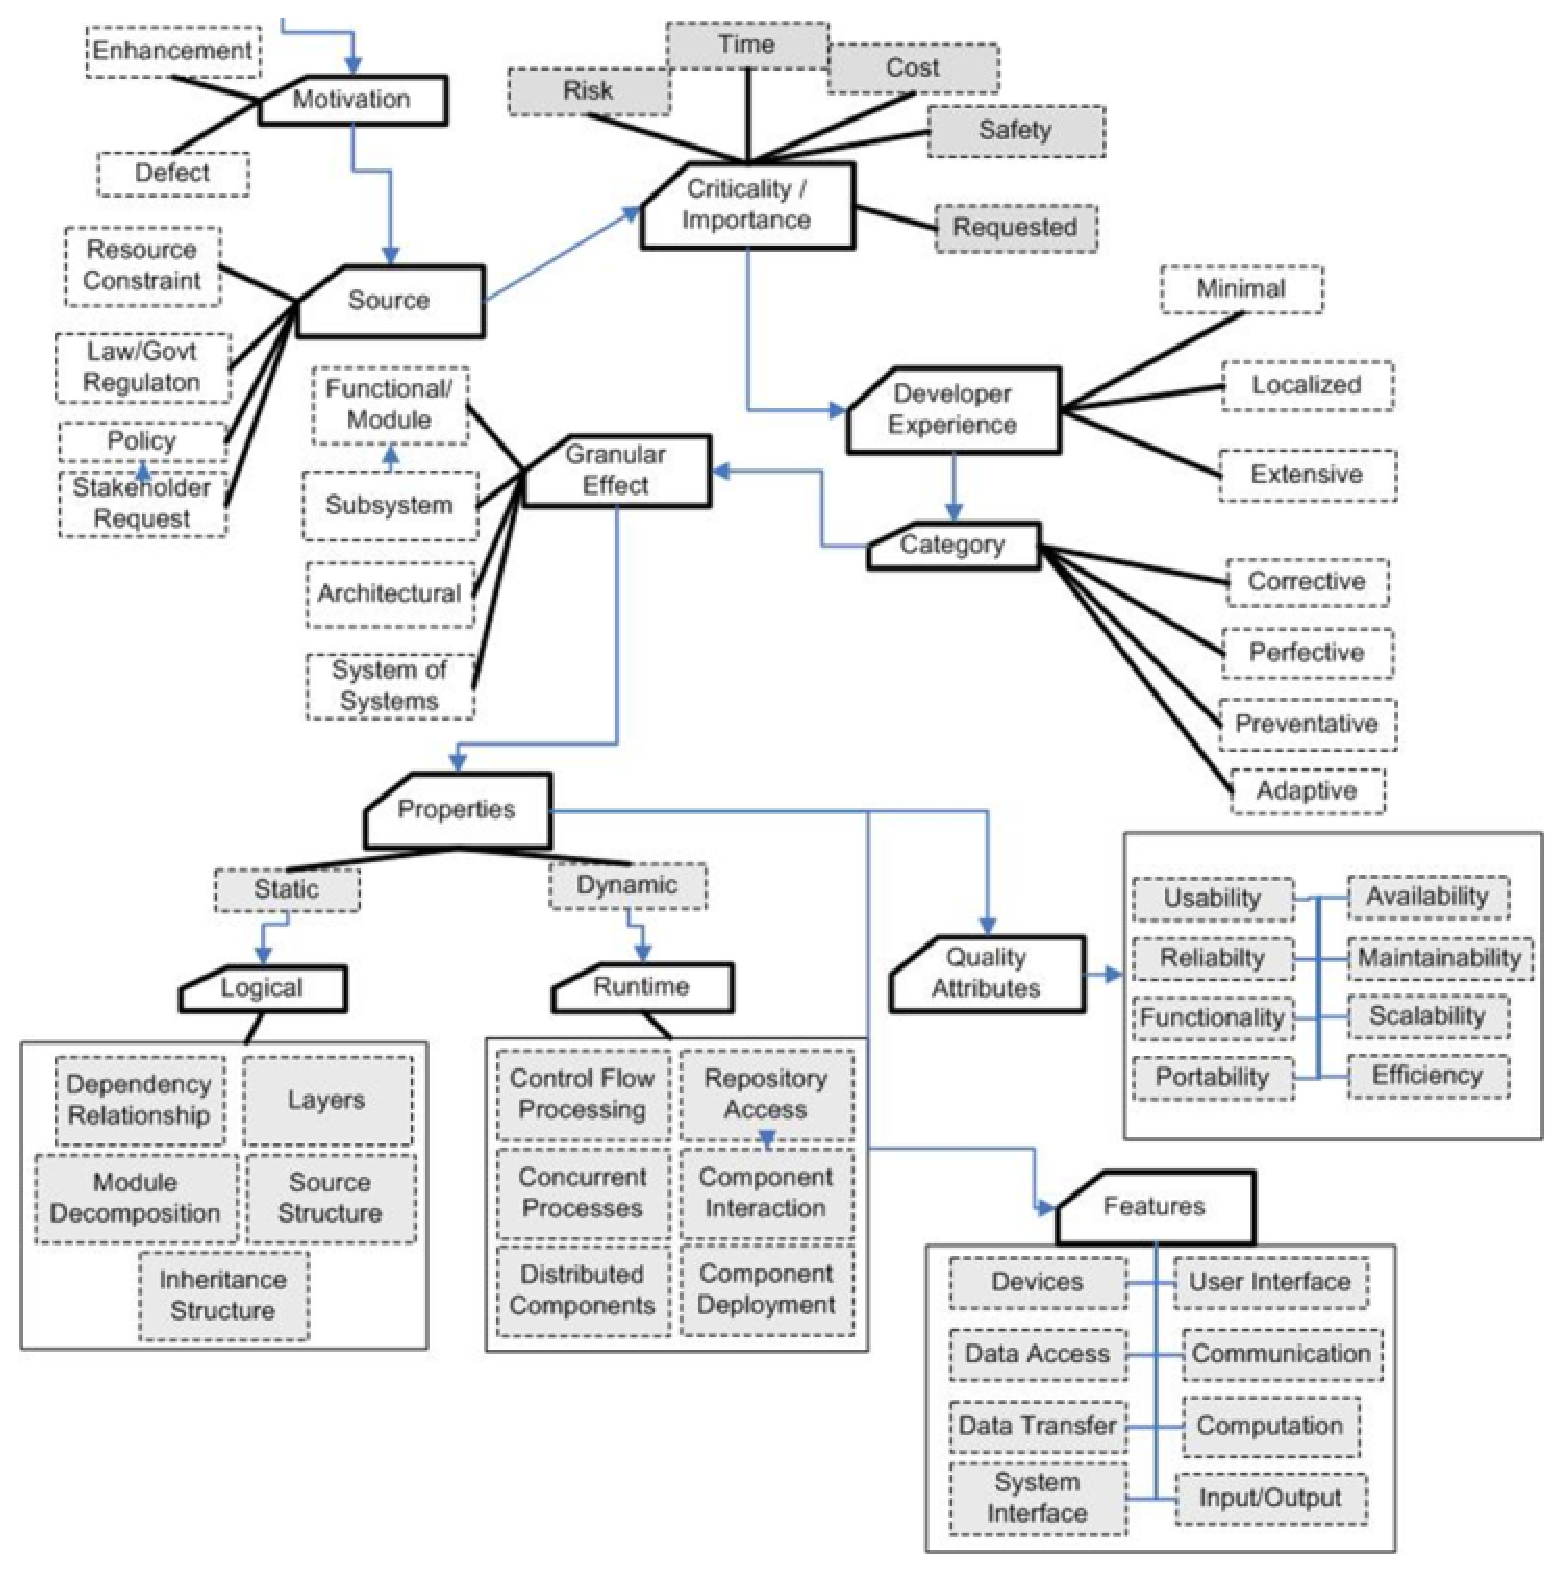
\includegraphics[width=0.8\textwidth]{img/saccs}
        \end{center}
      \end{figure}
  \end{slide}



%%%%%%%%%%%%%%%%%%%%%%%%%%%%%%%%%%%%%%%%%%%%%%%%%%%%%%%%%%%%%%%%%%%%%%%%%%%
\overlays{8}{%
  \begin{slide}[Box]{Research topic's matter}
    %    \vspace{-1cm}
    \textbf{Main results}
    \bi
    \fromSlide{1}{\item[{\includegraphics[width=.4cm]{red-bullet-on-white}}]Contribution}
    \bi
    \fromSlide{2}{\item Systematic review of software change}
    \fromSlide{3}{\item Software Architecture Change Characterization Scheme}
    \ei
    \ei
    \vspace{1cm}
    \fromSlide{4}{\textbf{Consequences :}}
    \bi
    \fromSlide{5}{\item [{\includegraphics[width=.4cm]{red-bullet-on-white}}]  Relevant results}
    % resultat pertinant grace a la sytematic review
    \fromSlide{6}{\item SACCS's strengh} 
    %Conséquence de ce processus, outil de qualité
    \fromSlide{7}{\item A usefull tool for developers} 
    % aide les developers a prendes des décisions
    \fromSlide{8}{\item An inovation} 
    % le premier du genre 
    \ei  
  \end{slide}
}

%% %% %%%%%%%%%%%%%%%%%%%%%%%%%%%%%%%%%%%%%%%%%%%%%%%%%%%%%%%%%%%%%%%%%%%%%%
%% \overlays{3}{%
%%   \begin{slide}[Wipe]{Using Join Point Interfaces (JPI)}
%%     \vspace{-1cm}
%%     \textbf{Dépendencies}
%%     \vspace{1cm}
%%     \begin{figure}
%%       \centering
%%       \onlySlide*{2}{ \vspace{0,5cm}  \hfill  \includegraphics[scale=0.35]{img/diag3ab.eps}}
%%       \onlySlide*{3}{     \includegraphics[scale=0.35]{img/diag3b.eps}}
%%     \end{figure}
%%   \end{slide}
%% }
%% %%%%%%%%%%%%%%%%%%%%%%%%%%%%%%%%%%%%%%%%%%%%%%%%%%%%%%%%%%%%%%%%%%%%%%
%% \overlays{2}{%
%% \begin{slide}[Wipe]{Polymorphic join points}
%%   \vspace{-1cm}
%%   \textbf{Example}
%%   \vspace{1cm}
%%   \begin{figure}
%%     \centering
%%     \includegraphics[scale=0.35]{img/dispatch.eps}
%%   \end{figure}
%%   \vspace{1cm}
%%   \bi
%%   \item
%%     \textit{Dispatch}
%%   \item 
%%  \fromSlide{2}{   Manual ?}
%%   \ei
%% \end{slide}
%% }
%% %% %%%%%%%%%%%%%%%%%%%%%%%%%%%%%%%%%%%%%%%%%%%%%%%%%%%%%%%%%%%%%%%%%%%%%
%% %


%% %% %%%%%%%%%%%%%%%%%%%%%%%%%%%%%%%%%%%%%%%%%%%%%%%%%%%%%%%%%%%%%%%%%%%%%%


\end{document}
